\usetikzlibrary{arrows.meta}

\begin{frame}{model for use-after-free}
    \begin{itemize}
        \item model for use-after-free, pointer is:
            \begin{itemize}
            \item allocated
            \item freed
            \item (other states?)
            \end{itemize}
        \item just track this logical state for each pointer
        \item ignore everything else
        \item assume all if statements/loop conditions can be true or false
    \end{itemize}
\end{frame}

\begin{frame}[fragile,label=useAfterFree1]{checking use-after-free (1)}
    \lstset{
        language=C,style=script,
        moredelim={**[is][\btHL<2>]{~2~}{~end~}},
    }
\begin{tikzpicture}
\node[anchor=north east] at (-.2, 0) {
\begin{lstlisting}
void someFunction(int foo, int bar) {
    int *quux = malloc(sizeof(int));
    // A
    ... /* omitted code that doesn't use quux */
    free(quux);
    // B
    ... /* omitted code that doesn't use quux */
    // C
    *quux = bar;
    ...
}
\end{lstlisting}
};

    \tikzset{flow/.style={draw,thick,font=\fontsize{9}{10}\selectfont,anchor=north west},
    flowLine/.style={thick,-Latex}}
    \begin{scope}[y=0.8cm]
        \node[flow,dashed] (A) at (0, 0) { A: quux: \textit{allocated} };
        \node[flow] (B) at (1, -1) { B: quux: \textit{freed} };
        \node[flow] (C) at (1, -2) { C (from \textit{freed}): USE-AFTER-FREE };
        \draw[flowLine] ([xshift=.5cm]A.south west) |- ([yshift=.1cm]B.west);
        \draw[flowLine] ([yshift=-.1cm]B.west) -- ++(-.2cm, 0cm) |- ([yshift=.1cm]C.west);
    \end{scope}
    
    \begin{visibleenv}<3->
        \node[draw=red,very thick,fill=white,align=center] at (0, -4) {
            analysis can give warning --- almost certainly bad
        };
    \end{visibleenv}
    \begin{visibleenv}<4->
        \node[draw=red,very thick,fill=white,align=center] at (0, -5) {
            exercise: how could this be a false positive?
        };
    \end{visibleenv}
\end{tikzpicture}
\end{frame}

\begin{frame}{result from clang's scan-build}
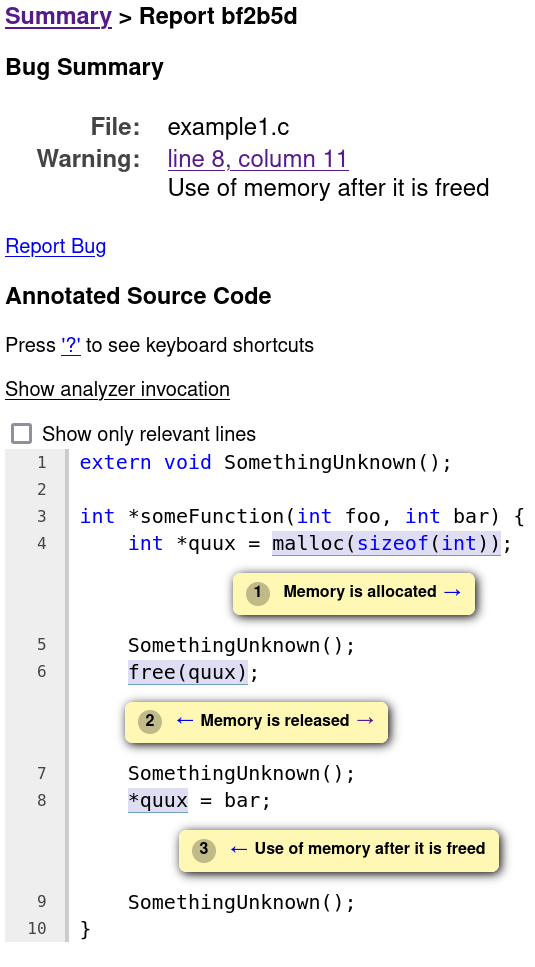
\includegraphics[height=0.9\textheight]{../static/scan-build-uaf-example1}
\end{frame}

\begin{frame}[fragile,label=useAfterFree2]{checking use-after-free (2)}
    \lstset{
        language=C,style=script,
        moredelim={**[is][\btHL<2>]{~2~}{~end~}},
    }
\begin{tikzpicture}
\node[anchor=north east] at (-.2, 0) {
\begin{lstlisting}
int *someFunction(int foo, int bar) {
    int *quux = malloc(sizeof(int));
    // A
    if (Complex(foo)) {
        free(quux);
        // B
    }
    ... /* omitted code that doesn't use quux */
    if (Complex(bar)) {
        // C
        *quux = bar;
    }
    ... /* omitted code that doesn't use quux */
    // D
}
\end{lstlisting}
};

    \tikzset{flow/.style={draw,thick,font=\fontsize{9}{10}\selectfont,anchor=north west},
    flowLine/.style={thick,-Latex}}
    \begin{scope}[y=0.8cm]
        \node[flow,dashed] (A) at (0, 0) { A: quux: \textit{allocated} };
        \begin{visibleenv}<2->
            \node[flow] (B) at (1, -1) { B: quux: \textit{freed} };
        \end{visibleenv}
        \begin{visibleenv}<3->
            \node[flow] (C1) at (1, -2) { C (from quux \textit{freed}): USE-AFTER-FREE };
        \end{visibleenv}
        \begin{visibleenv}<2->
            \node[flow] (D1) at (2, -3) { D (from quux \textit{freed})};
        \end{visibleenv}
        \begin{visibleenv}<4->
            \node[flow] (C2) at (1, -4) { C (from quux \textit{allocated}): ok };
            \node[flow] (D2) at (2, -5) { D (from allocated)};
        \end{visibleenv}
        \begin{visibleenv}<2->
            \draw[flowLine] ([xshift=.5cm]A.south west) |- ([yshift=.1cm]B.west);
        \end{visibleenv}
        \begin{visibleenv}<3->
            \draw[flowLine] ([yshift=-.1cm]B.west) -- ++(-.4cm, 0cm) |- ([yshift=.1cm]C1.west);
        \end{visibleenv}
        \begin{visibleenv}<2->
            \draw[flowLine] ([yshift=-.1cm]B.west) -- ++ (-.4cm,0cm) |- ([yshift=.1cm]D1.west);
        \end{visibleenv}
        \begin{visibleenv}<4->
            \draw[flowLine] ([xshift=.5cm]A.south west) |- ([yshift=.1cm]C2.west);
            \draw[flowLine] ([yshift=-.1cm]C2.west) -- ++(-.2cm,0cm) |- ([yshift=.1cm]D2.west);
            \draw[flowLine] ([xshift=.5cm]A.south west) |- ([yshift=.1cm]D2.west);
        \end{visibleenv}
    \end{scope}
    
    \begin{visibleenv}<4->
        \node[draw=red,very thick,fill=white,align=center,anchor=north west] at (-8, -6) {
            one idea: guess that Complex(foo) can be probably be true \\
            ~ \\
            option 1: say ``something wrong maybe''? \\
            option 2: try to figure out if Complex(foo) is true?)
        };
    \end{visibleenv}
\end{tikzpicture}
\end{frame}


\begin{frame}{result from clang's scan-build}
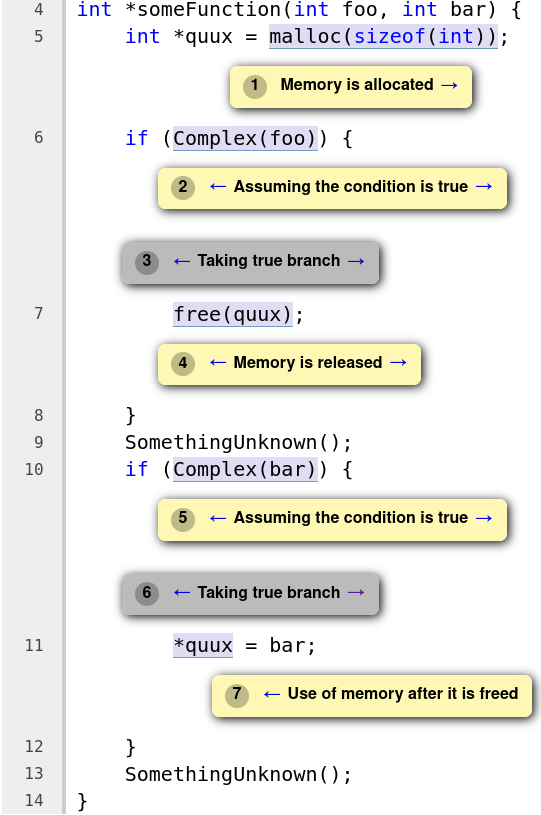
\includegraphics[height=0.9\textheight]{../static/scan-build-uaf-example2}
\end{frame}

